% \section{Testing und Laufzeitanalyse}
% \label{sec:testing_und_laufzeitanalyse}

% \subsection{Testing}
% \label{ssec:testing}
\section{Testing}
\label{sec:testing}

\subsection{Testfälle}
\label{ssec:testfaelle}

% Beschreibung der Testfälle
Die Testfälle sind in Abbildung \ref{tab:testcases} aufgelistet.

Die konkreten Testdateien sind in \ref{sec:testdateien} aufgelistet.

\begin{figure}[H]
    \centering
    % unterteilt nach Normalfällen, Grenzfällen, Fehlerfällen
    \begin{tabular}{|l|l|l|}
        \hline
        \textbf{Testfall}                 & \textbf{Beschreibung}                  & \textbf{Bemerkung}      \\
        \hline
        \hline
        \textbf{Normalfälle}              &                                        &                         \\
        \hline
        \texttt{IHK\_1}                   & IHK-Beispiel 1                         &                         \\
        \texttt{IHK\_2}                   & IHK-Beispiel 2                         &                         \\
        \texttt{spiral}                   & \enquote{Spiralförmige} Bewegung       &                         \\
        \texttt{single}                   & Eine einzige Bewegung                  &                         \\
        \hline
        \hline
        \textbf{Grenzfälle}               &                                        &                         \\
        \hline
        \texttt{diagonals}                & Bewegung zwischen Eckpunkten           &                         \\
        \texttt{edges}                    & Bewegung am Rand                       &                         \\
        \texttt{multiple\_per\_step}      & Mehrere Instruktionen in Zeitintervall &                         \\
        \texttt{multiple\_simultaneously} & Mehrere Instruktionen gleichzeitig     &                         \\
        \texttt{same\_dest}               & Instruktionen mit gleichem Ziel        &                         \\
        \hline
        \hline
        \textbf{Fehlerfälle}              &                                        &                         \\
        \hline
        \texttt{invalid\_dim}             & \texttt{dim} ungültig                  & Koordinate kleiner 0    \\
        \texttt{invalid\_vmax}            & \texttt{vmax} ungültig                 & \texttt{vmax} kleiner 0 \\
        \texttt{invalid\_amax}            & \texttt{amax} ungültig                 & \texttt{amax} kleiner 0 \\
        \texttt{invalid\_freq}            & \texttt{freq} ungültig                 & \texttt{freq} kleiner 0 \\
        \texttt{invalid\_instruction}     & Ungültige Instruktion                  & Koordinate außerhalb    \\
        \texttt{invalid\_no\_instruction} & Keine Instruktion                      &                         \\
        \hline
    \end{tabular}
    \caption{Testfälle}
    \label{tab:testcases}
\end{figure}

\subsection{Beobachtungen}
\label{ssec:beobachtungen}

% Beschreibung der Beobachtungen
Für alle definierten Testfälle wurden die Ergebnisse mit den erwarteten Ergebnissen verglichen.
Es konnte kein Fehlverhalten festgestellt werden.
Das bedeutet:
\begin{itemize}
    \item Fehlerfälle wurden korrekt erkannt und abgefangen.
    \item Grenz- und Normalfälle wurden korrekt berechnet.
\end{itemize}

Einige Ergebnisse sind in den folgenden Abbildungen dargestellt.

% \foreach \file in {IHK_1, IHK_2, test_spiral, test_diagonals, test_edges, test_multiple_per_step, test_multiple_simultaneously}
\foreach \file/\fileEscaped in {IHK_1/IHK\_1, IHK_2/IHK\_2, test_spiral/spiral, test_diagonals/diagonals, test_edges/edges, test_multiple_per_step/multiple\_per\_step, test_multiple_simultaneously/multiple\_simultaneously, test_same_dest/test\_same\_dest}
    {
        \begin{figure}[H]
            \centering
            % two subfigures side by side
            \begin{subfigure}[b]{0.45\textwidth}
                \centering
                \includegraphics[width=\textwidth]{../python/output/\file_cam_pos.png}
                \caption{Bewegung der Spidercam für Test \texttt{\fileEscaped}}
            \end{subfigure}
            \hfill
            \begin{subfigure}[b]{0.45\textwidth}
                \centering
                \includegraphics[width=\textwidth]{../python/output/\file_rope_lengths.png}
                \caption{Veränderung der Seillängen für Test \texttt{\fileEscaped}}
            \end{subfigure}
            \caption{Ergebnisse für Test \texttt{\fileEscaped}}
        \end{figure}
    }

Besonders interessant sind die letzten beiden Beispiele.
Hier wird deutlich, dass die Spidercam auch bei mehreren gleichzeitig auftretenden Bewegungen korrekt funktioniert.

% \subsection{Laufzeitanalyse}
% \label{ssec:laufzeitanalyse}

% % Beschreibung der Laufzeitanalyse
% Die Laufzeitanalyse wurde mit $\ldots$ durchgeführt.
% Jeder Testfall wurde $\ldots$ mal ausgeführt und im Anschluss die Laufzeiten gemittelt.

% Für die einzelnen Testfälle aus Tabelle \ref{tab:example_testcases} ergeben sich die Laufzeiten in Tabelle \ref{tab:example_runtime}.

% \begin{figure}[H]
%     \centering
%     % unterteilt nach Normalfällen, Grenzfällen, Fehlerfällen
%     % median, mean, standard deviation
%     \begin{tabular}{|l|l|l|l|}
%         \hline
%         \textbf{Testfall}    & \textbf{Median} & \textbf{Mittelwert} & \textbf{Standardabweichung} \\
%         \hline
%         \hline
%         \textbf{Normalfälle} &                 &                     &                             \\
%         \hline
%         \hline
%         \textbf{Grenzfälle}  &                 &                     &                             \\
%         \hline
%         \hline
%         \textbf{Fehlerfälle} &                 &                     &                             \\
%         \hline
%     \end{tabular}
%     \caption{Beispiel für eine Tabelle mit Laufzeiten}
%     \label{tab:example_runtime}
% \end{figure}

% % graphische Darstellung der Laufzeiten
% \begin{figure}[H]
%     \centering
%     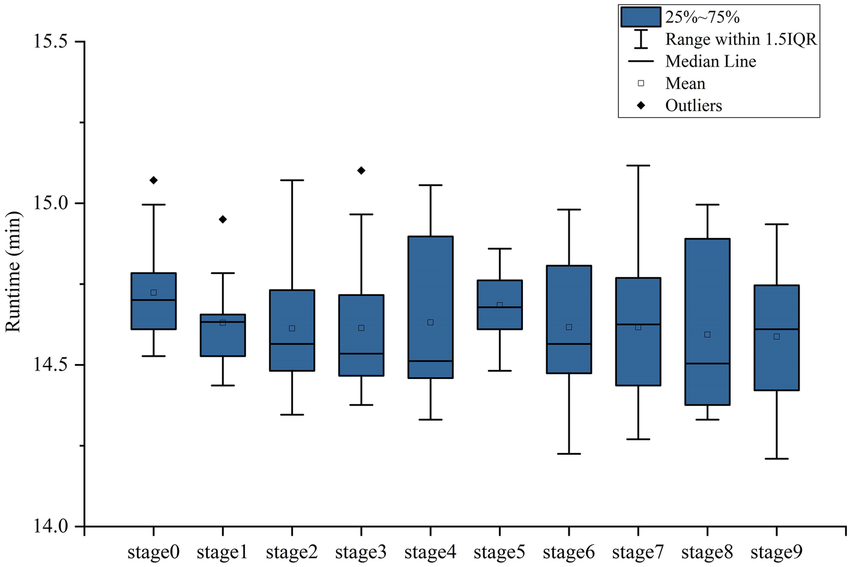
\includegraphics[width=0.8\textwidth]{figures/example_runtime.png}
%     \caption{Beispiel für eine graphische Darstellung der Laufzeiten}
%     \label{fig:example_runtime}
% \end{figure}

% Besonders auffällig ist $\ldots$, da der Algorithmus in $\mathcal{O}(n^m)$ läuft.

% Für den praktischen Einsatz muss die Laufzeit nochmals verbessert werden.
% Siehe dazu Abschnitt \ref{ssec:ausblick}.